\section{Introduction}

    Engin Pas Tangible est un moteur graphique reposant sur le principe de Ray Marching : un système de 3D similaire au Ray Tracing, mais beaucoup plus rarement utilisé. Ce système a certains avantages par rapport au Ray Tracing, comme par exemple de permettre une implémetation peu coûteuse de fractales, ou autres figures se reproduisant à l'identique. \\
    Le Ray Marching repose sur la projection de rayons depuis une camera vers la scene. Pour projeter ces rayons, on les fait avancer pas à pas (\emph{Marching}), avec la distance d'un pas dependant de la distance à la scene 3D.
\\
\\
%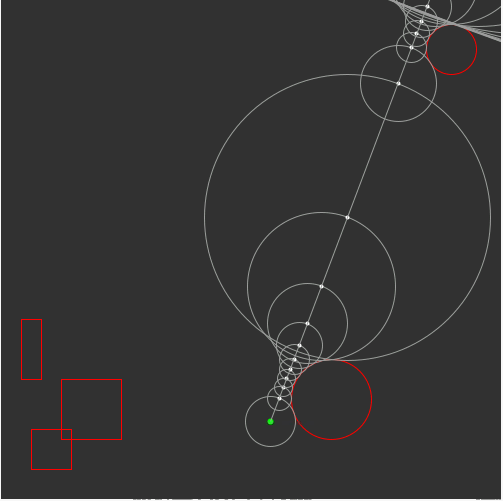
\includegraphics[width=8cm]{images/marching.png}
\begin{figure}[h]
    \centering
    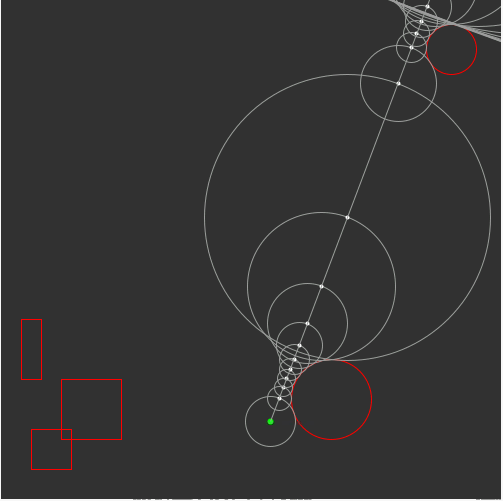
\includegraphics[width=8cm]{images/marching.png}
    \caption{Illustration 2D de la marche d'un rayon (on expliquera plus en detail dans \ref{subsec:projection} \nameref{subsec:projection})}
    \label{fig:my_label}
\end{figure}
